\documentclass[12pt,a4paper,titlepage,oneside,BCOR1cm]{scrreprt}

\usepackage{ngerman} % neue deutsche Rechtschreibung
\usepackage[latin1]{inputenc}
\usepackage[english]{babel} % Silbentrennung
\usepackage{amsmath,amstext,amssymb}

\usepackage{setspace} % 1,5 Zeilenabstand
\onehalfspacing
\usepackage[T1]{fontenc} 
\usepackage{bibgerm}
\pagestyle{headings}


\usepackage{ulem}
\normalem %�nderung von \em und \emph nicht zulassen

\usepackage{graphicx} % Bilder einf�gen
\usepackage{color} % Farben
\usepackage{subfigure} % mehrere Abbildungen nebeneinander/�bereinander
\usepackage{latexsym}
\usepackage{fancyhdr} %Kopf- und Fu�zeilen
\bibliographystyle{gerunsrt} % Literaturangaben nach Auftreten sortieren %{gerplain}

\usepackage[pagebackref,pdfpagelabels]{hyperref} %Hyperlinks zw. Textstellen

\usepackage{multirow}



%%%%%%%%%%%%%%%%%%%%%%%%%%%%%%%%%%%%%%%%%%%%%%%%%%%%%%%%%%%%%%%%%%%%%%%%%%%%%%%%%%%%%%%%%%%%%%
% Hier bitte Werte �ndern %%%%%%%%%%%%%%%%%%%%%%%%%%%%%%%%%%%%%%%%%%%%%%%%%%%%%%%%%%%%%%%%%%%%
\date{\today} %{September 2006}
\author{DAI-Labor}
\title{Dokumentenvorlage f�r ein Diplomarbeitsproposal} % Bitte unter chapter/deckblatt.tex �ndern!!
%%%%%%%%%%%%%%%%%%%%%%%%%%%%%%%%%%%%%%%%%%%%%%%%%%%%%%%%%%%%%%%%%%%%%%%%%%%%%%%%%%%%%%%%%%%%%%

%Beginn des Dokuments
\begin{document}
%\maketitle

\pagenumbering{Roman} % R�mische Aufz�hlung
\thispagestyle{empty}
\begin{figure}[htbp]
	\centering
 \begin{minipage}[b]{41 mm}
   %\includegraphics[width=40 mm]{figures/AOT-Logo.png}
   %\includegraphics[width=40 mm]{figures/DAI_Logo_engl.png}
   
\includegraphics[width=40 mm]{figures/DAI_Logo.png}
 \end{minipage}
% \begin{minipage}[b]{73 mm}
% \includegraphics[width=72 mm]{figures/FakAOT2.png}
% \end{minipage}
% \begin{minipage}[b]{30 mm}
%  \includegraphics[width=30mm]{figures/TU2.png}
% \end{minipage}
\end{figure}

~\vspace{0.5cm}

\begin{center}
\begin{Huge}
Technische Universit�t Berlin\\
\vspace{1mm}
\end{Huge}{\Large Fakult�t IV - Elektrotechnik und Informatik\\
Fachgebiet AOT\\
Prof. Dr. Sahin Albayrak}\\

\vspace{26mm}
\begin{LARGE}
Masterarbeitsproposal\\
\end{LARGE}
\vspace{8mm}
\begin{LARGE}
Gesture Recognition for Human-Robot Interaction:\\
An approach based on skeletal points tracking using depth camera \\
\end{LARGE}
\vspace{3 cm}
Sivalingam Panchadcharam Aravinth\\
Matrikel--Nummer 342899\\
me@aravinth.info\\
\vspace{1cm}
\begin{tabular}{lll}
{\bf Betreuer} & Dr. Yuan Xu \\
\end{tabular}

\end{center}
%\clearpage

 % Titelseite
\tableofcontents % Inhaltsverzeichnis
\addcontentsline{toc}{chapter}{Index} % Auch Inhaltsverzeichnis aufnehmen
\newpage
%%%%%%%%%%%%%%%%%%%%%%%%%%%%%%%%%%%%%%%%%%%%%%%%%%%%%%%%%%%%%%%%%%%%%%%%%%%%%%%%%%%%%%%%%%%%%%

% Hauptteil
\pagenumbering{arabic} % Normale Aufz�hlung
\chapter{Abstract} Human-robot interaction (HRI) has been a topic of both science fiction and academic speculation even before any robots existed. HRI research is focusing to build an intuitive, and easy communication with the robot through speech, gestures, and facial expressions. The use of hand gestures provides an attractive alternative to complex interfaced devices for HRI. In particular, visual interpretation of hand gestures can help in achieving the ease and naturalness desired for HRI. This has motivated a very active research area concerned with computer vision-based analysis and interpretation of hand gestures. Important differences in the gesture interpretation approaches arise depending on whether static model of the gesture or non-static model of the gesture is used. 

In this thesis, we attempt to do the method of modeling, analyzing, and recognizing gestures by using Computer Vision and Machine Learning techniques. Furthermore, Static (Gesture is formed by non-moving appearance of body parts) and non-static gestures (Gesture is formed by moving appearance of body parts), will be used to interact with robot and command the robot to execute certain actions.

We further hope to provide a platform to integrate Sign Language Translation to assist people with hearing and speech disabilities. However, further implementations and training data are needed to use this platform as a full fledged Sign Language Translator.

\chapter{Motivation} Huge influence of computers in society has made smart devices, an important part of our lives. Availability and affordability of such devices motivated us to use them in our day-to-day living. 

Interaction with smart devices has still been mostly by displays, keyboards, mouse and touch interfaces. These devices have grown to be familiar but inherently limit the speed and naturalness with which we can interact with the computer. 

The list of smart devices includes personal automatic and semi-automatic robots which are also playing a major role in our household. For an instance, Smart Vacuum Cleaner is an robot that automatically cleans the floor and goes to its charging station without human interaction. Usage of robots for domestic and industrial purposes have been continuously increasing. Thus in recent years there has been a tremendous push in research toward an intuitive, and easy communication with the robot through speech, gestures, and facial expressions.

Tremendous progress had been made in speech recognition, and several commercially successful speech interfaces have been deployed. However, there has been an increased interest in recent years in trying to introduce other human-to-human communication modalities into HRI. This includes a class of techniques based on the movement of the human arm and hand, or hand gestures. The use of hand gestures provides an alternative mode of communication for Human-robot interaction (HRI) than the conventional interfaced devices.

\chapter{Background} 
\section{Robot and Artificial intelligence} Proper vision is of the utmost importance for the function of any vision based autonomous robot. Areas of artificial intelligence deal with autonomous planning or deliberation for robotical systems to navigate through an environment. A detailed understanding of these environments is required to navigate through them. Information about the environment could be provided by a computer vision system, acting as a vision sensor and providing high-level information about the environment and the robot.

Computer vision is a field that includes methods for acquiring, processing, analyzing, and understanding images and, in general, high-dimensional data from the real world in order to produce numerical or symbolic information, e.g., in the forms of decisions.

In this thesis, we will focus on the hand gesture recognition using computer vision techniques for a humanoid robot name as NAO.

Nao is an autonomous, programmable humanoid robot developed by Aldebaran Robotics. The Nao Academics Edition was developed for universities and laboratories for research and education purposes.
\begin{table}
	[h] \centering \caption{Nao's hardware specification } \label{tb:interf:1} 
	\begin{tabular}
		{|l|l|} \hline Height & 58 centimetres (23 in) \\
		\hline Weight & 4.3 kilograms (9.5 lb) \\
		\hline Autonomy & 60 minutes (active use), 90 minutes (normal use) \\
		\hline Degrees of freedom & 21 to 25 \\
		\hline CPU & 2 x Intel Atom @ 1.6 GHz \\
		\hline Built-in OS & Linux \\
		\hline Compatible OS & Windows, Mac OS, Linux \\
		\hline Programming languages & C++, Python, Java, MATLAB, Urbi, C, .Net \\
		\hline Vision & 2 x HD 1280x960 cameras \\
		\hline Connectivity & Ethernet, Wi-Fi \\
		\hline \multirow{6}{*}{Sensors} & 4 x directional microphones \\
		& 1 x sonar rangefinder \\
		& 2 x IR emitters and receivers \\
		& 1 x inertial board \\
		& 9 x tactile sensors \\
		& 8 x pressure sensors \\
		\hline 
	\end{tabular}
\end{table}

\subsection{NAO Vision} Two identical video cameras are located in the forehead. They provide a up to 1280x960 resolution at 30 frames per second. They can be used to identify objects in the visual field such as goals and balls, and bottom camera can ease NAO?s dribbles. NAO contains a set of algorithms for detecting and recognizing faces and shapes. NAO can recognize who is talking to it or find a ball or, eventually, more complex objects.

\subsection{Extending NAO with Depth Camera} 
3D cameras such as Microsoft Kinect and Asus Xtion are used not only for gaming but also for analyzing 3D data, including algorithms for feature selection, scene analysis, motion tracking, skeletal tracking and gesture recognition. 

In this thesis, we focus on using Asus Xtion as an external hardware to be used with NAO due to the computational limitations of the NAO to process the images from two inbuilt hd stereo cameras, that ultimately makes NAO incapable of doing an efficient gesture recognition in real time.

\begin{table}
	[h] \centering 
	\begin{tabular}
		{ll} 
		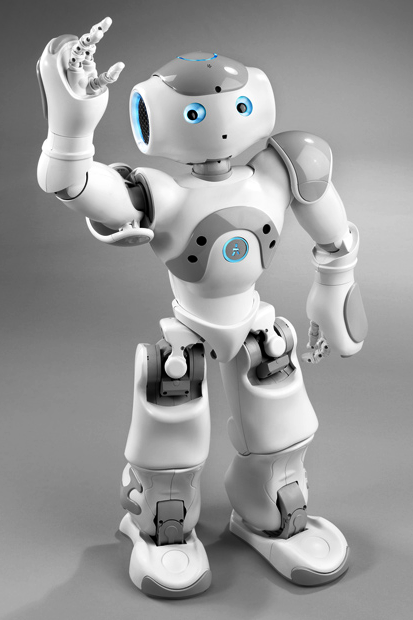
\includegraphics[height=7cm]{figures/nao.png} & 
		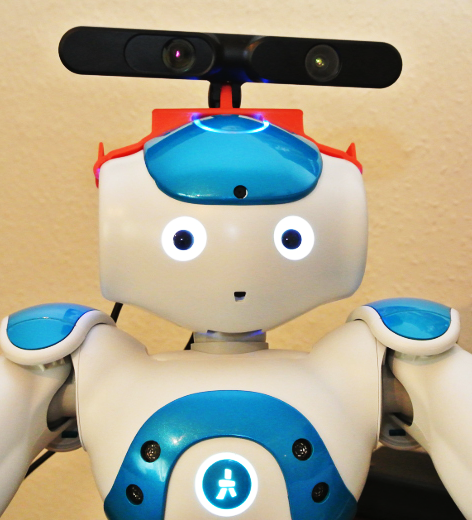
\includegraphics[height=7cm]{figures/nao-xtion.png} \\
		NAO & Asus Xtion on NAO 
	\end{tabular}
\end{table}

\section{Hand Gesture} Human hand gestures are a means of non-verbal interaction among people. They range from simple actions of using our hand to point at to the more complex ones that express our feelings and allow us to communicate with others. To exploit the use of gestures in HRI it is necessary to provide the means by which they can be interpreted by robots. The HCI interpretation of gestures requires that dynamic and/or static configurations of the human hand, arm, and even other parts of the human body, be measurable by the machine. 

\section{Hand Gesture Recognition} Initial attempts to recognize hand gestures, resulted in electro-mechanical devices that directly measure hand and/or arm joint angles and spatial position using sensors. Glove-based gestural interfaces require the user to wear such a complex device that hinders the ease and naturalness with which the user can interact with the computer controlled environment. 

Even though such hand gloves are used in highly specialized domain such as simulation of medical surgery or even the real surgery, the everyday user will be certainly deterred by such a sophisticated interfacing devices. As an active result of the motivated research in HCI, computer vision based techniques were innovated to augment the naturalness of interaction.

\subsection{Gesture Modeling} Gesture modeling depends primarily on the intended application. For an application that needs just hand gesture to go up and down or left and light, a very simple model may be sufficient. However, if the purpose is a natural-like interaction, a model has to be sophisticated enough to interpret all the possible gesture. The following section discusses various gesture modeling techniques which are being used by the existing hand gesture recognition applications. 

\begin{figure}
	[h] \centering 
	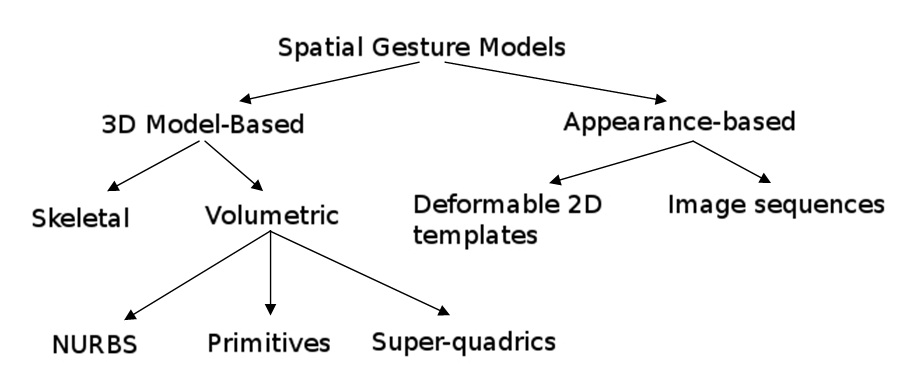
\includegraphics[height=6cm]{figures/ges-model.png} 
	\caption{Different gesture modeling} 
	\label{fig:ges:model} 
\end{figure}

Appearance based models don't use a spatial representation of the body anymore, because they derive the parameters directly from the images or videos using a template database. 

3D Hand model approach can use volumetric or skeletal models, or even a combination of the two. Volumetric approaches have been heavily used in computer animation industry and for computer vision purposes. The models are generally created of complicated 3D surfaces. The drawback of this method is that is very computational intensive. 

Instead of using intensive processing of the 3D models and dealing with a lot of parameters, one can just use a simplified version of joint angle parameters along with segment lengths. This is known as a skeletal representation of the body, where a virtual skeleton of the person is computed and parts of the body are mapped to certain segments. The analysis here is done using the position and orientation of these segments and the relation between each one of them.

In this thesis, we focus on Skeletal based modeling algorithms which are faster because the detection program to focus on the significant parts of the body. Moreover, it allows to do pattern matching against a template database. 


\subsection{Gestural Taxonomy }
Several alternative taxonomies have been suggested that deal with psychological aspects of gestures. All hand/arm movements are first classified into two major classes as shown in the figure \ref{fig:ges:tax}.

\begin{figure}
	[h] \centering 
	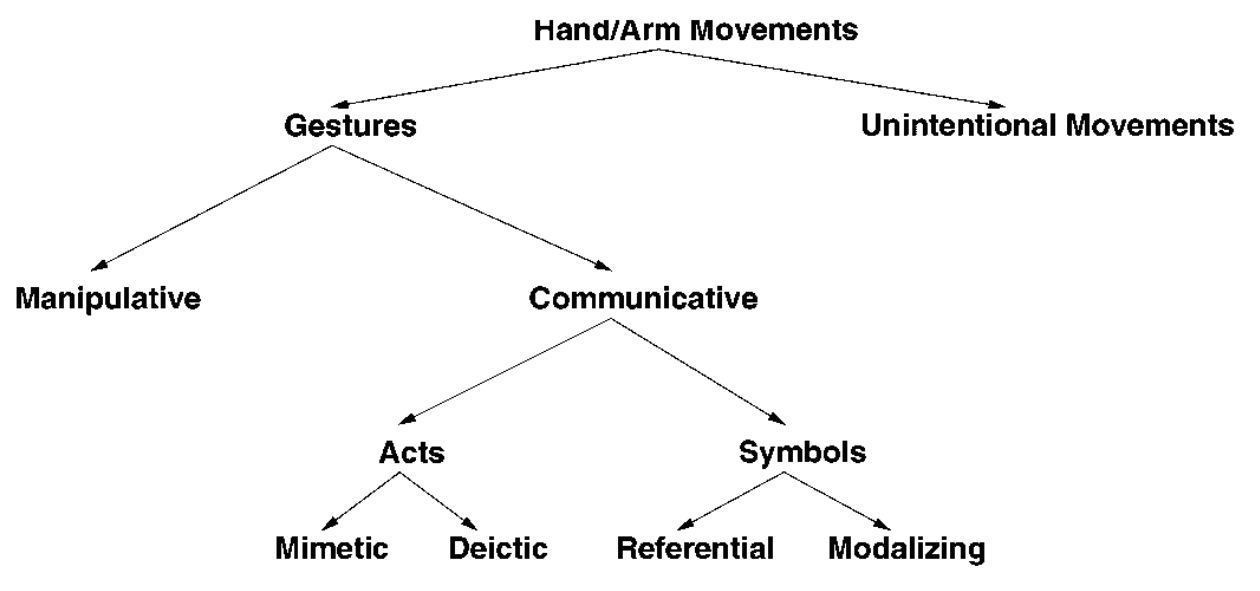
\includegraphics[height=7cm]{figures/ges-tax.png} 
	\caption{Different gesture modeling} 
	\label{fig:ges:tax} 
\end{figure}

Manipulative gestures are the ones used to act on objects. For example moving a chair from one location to another. Manipulative gestures in the context of HRI are mainly developed for medical surgery. Communicative gestures, on the other hand, have purely communicational purpose. In a natural environment they are usually accompanied by speech or spoken as a sign language. In HRI context these gesture are one of the commonly used gestures, since they can often be represented by static as well as dynamic hand postures.

In this thesis, we focus on communicative gestures in the form of symbols. They symbolize some referential action. For instance, circular motion of index finger may be a referred as an alphabet "O" or as an object such as wheel or as a command to turn in a circular motion .


\subsection{Gesture Recognition}
The task of gesture recognition shares certain similarities with other recognition tasks, such as speech recognition and biometrics. Though alternatives such as  DP-matching algorithms have been attempted, the most successful solutions involves feature-based statistical learning algorithm, usually Hidden Markov Models. 

In this thesis, we focus on the recognition technique based on hidden Markov model (HMM) that is a statistical model in which the system being modeled is assumed to be a Markov process with unobserved (hidden) states. In simpler Markov models, the state is directly visible to the observer, and therefore the state transition probabilities are the only parameters. In a hidden Markov model, the state is not directly visible, but output, dependent on the state, is visible.


\chapter{Goal} As described earlier, HRI research is focusing to build an intuitive, and easy communication with the robot through speech, gestures, and facial expressions. The use of hand gestures provides the ease and naturalness with which the user can interact with robots.

In this thesis, we attempt to implement a feature for NAO to recognize hand gestures and execute a predefined action based on the gesture. 

In order to achieve this, NAO will be extended with an external Depth Camera, that will enable NAO to recognize static as well as dynamic gestures. This 3D camera will be mounted on the head of NAO, so that it can scan for gestures in the horizon. 

With the hand gesture recognizing feature, NAO will be available to the users in two modes a) Command mode b) Translation mode.

In command mode, a gesture will be recognized by NAO and related task will be executed. Even though the gesture based Interaction is real time, NAO can not be interrupted or stopped by using any gesture while it is executing a task. However, part of NAO intelligence such as voice commands can be used in such situation to stop or interrupt the ongoing task execution.

In translation mode, NAO will be directly translating the meaning of the trained gestures. To achieve this, text-to-speech SDK of NAO will be used and translated gesture can be said out loud using the integrated speaker. This feature of NAO will be allowing it to translate a sign language to assist people with hearing and speech disabilities.

In this thesis, we planned to train NAO with few very simple gestures due to the reason that NAO has limited resources. Gestures will involve both the hands or single hand to interact with the robot.

\chapter{Task} The figure \ref{fig:flow} shows the flow diagram of hand gesture recognition. Each block contains submodules which are processed by different software components.
\begin{figure}
	[h] \centering 
	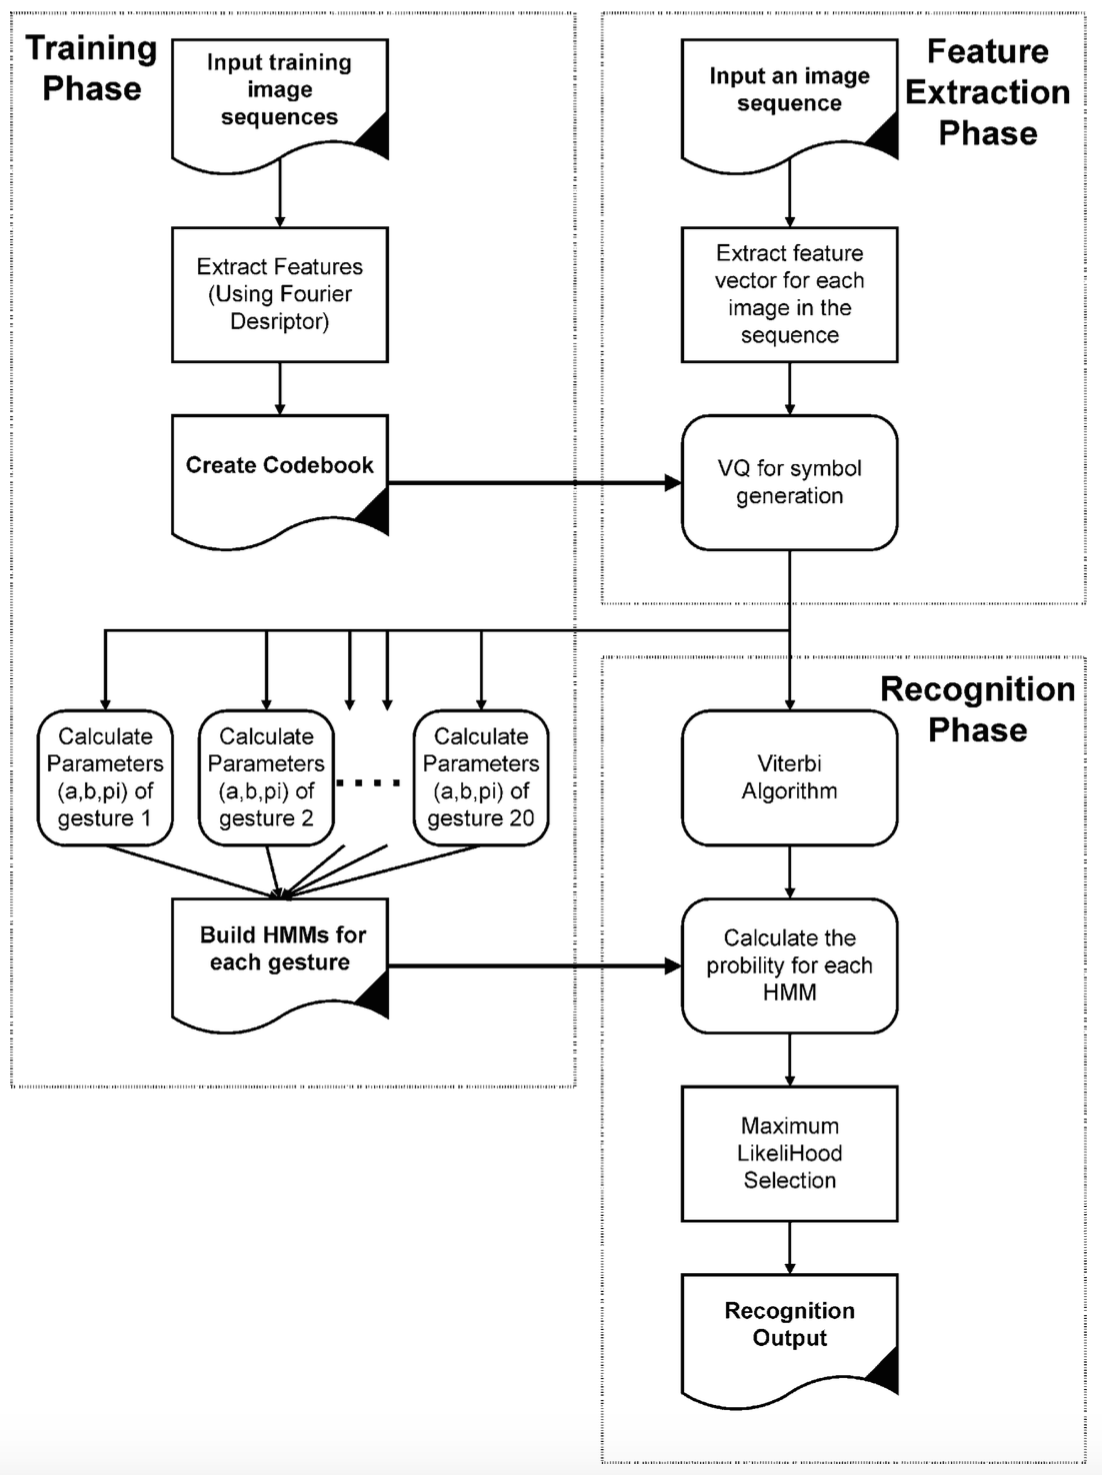
\includegraphics[height=10cm]{figures/flow.png} \caption{Flow diagram of hand gesture recognition system} \label{fig:flow} 
\end{figure}

\section{Sense} Sensor data from the 3D camera as images as shown in the figure 1, will be sent to Feature Detection module that will track the anatomical landmarks of the human body to extract the features as shown in the figure 2
\begin{table}
	[h] \centering 
	\begin{tabular}
		{ll} 
		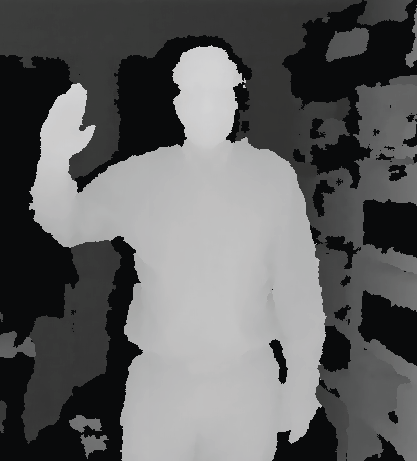
\includegraphics[height=7cm]{figures/depth.png} & 
		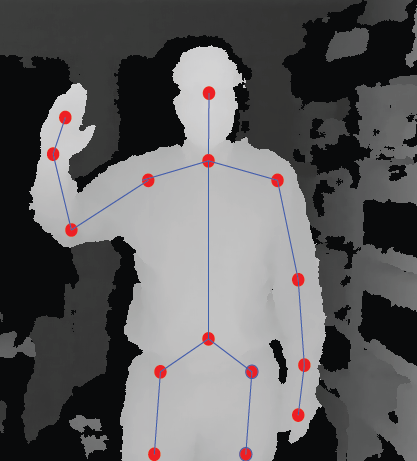
\includegraphics[height=7cm]{figures/depth-skeleton.png} \\
		Depth image of 3D Camera & Skeleton tracking 
	\end{tabular}
\end{table}

\section{Feature Extraction}

\section{Classification}
\begin{table}
	[h] \centering 
	\begin{tabular}
		{ll} 
		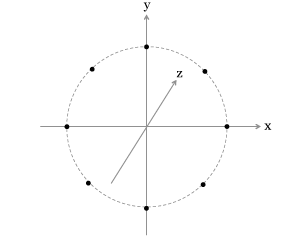
\includegraphics[width=6cm]{figures/ges-states.png} & 
		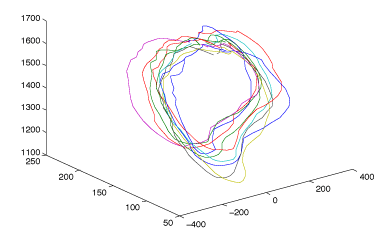
\includegraphics[width=10cm]{figures/ges-train.png} \\
		States & Training 
	\end{tabular}
\end{table}

\section{Gesture Analysis and Recognition}
\begin{figure}
	[h] \centering 
	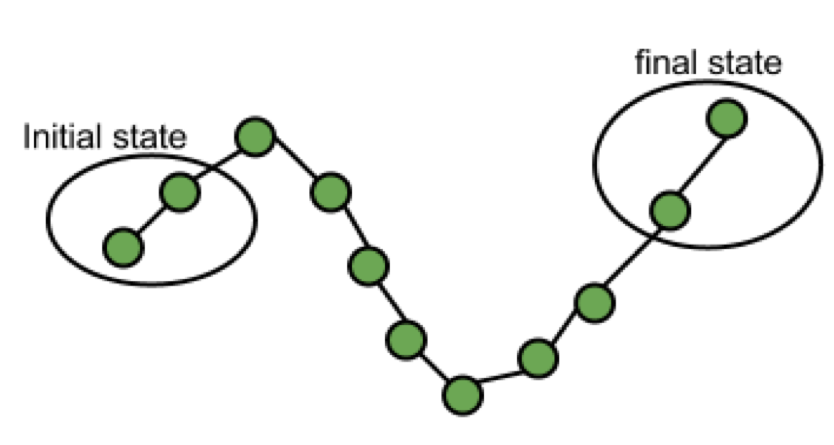
\includegraphics[height=7cm]{figures/ges-rec.png} \caption{ hand gesture recognition} \label{fig:ges:reg} 
\end{figure}



\newpage

%�bernehme alle Referenzen aus chapter/bibliography.bib
\nocite{*}
\bibliography{chapter/bibliography} % Literaturverzeichnis
\addcontentsline{toc}{chapter}{Bibliography}
%\appendix % andere Aufz�hlung
%%%%%%%%%%%%%%%%%%%%%%%%%%%%%%%%%%%%%%%%%%%%%%%%%%%%%%%%%%%%%%%%%%%%%%%%%%%%%%%%%%%%%%%%%%%%%%
% Hier kommen die Anh�nge %%%%%%%%%%%%%%%%%%%%%%%%%%%%%%%%%%%%%%%%%%%%%%%%%%%%%%%%%%%%%%%%%%%%
%\include{chapter/anhanga}
%\include{chapter/anhangb}
\end{document}

